\documentclass[conference]{IEEEtran}
\usepackage[utf8]{inputenc}
\usepackage[T1]{fontenc}
\usepackage[spanish,es-noshorthands,es-tabla]{babel}
\usepackage{amsmath,amssymb}
\usepackage{graphicx}
\usepackage{booktabs}
\usepackage{multirow}
\usepackage{xcolor}
\usepackage{url}
\usepackage{cite}
\graphicspath{{figuras/}{figuras/pilares/}{figuras/top_policies/}{figuras/imitacion/}}
\newcommand{\G}{G_0}

\begin{document}

\title{Control jerárquico con RL profundo, PBRS e imitación\\ en RoboCup 2D: persecución, conducción y definición}

% Completar con todos los integrantes del equipo.
\author{\IEEEauthorblockN{Fabricio Chávez}
\IEEEauthorblockA{Curso de Aprendizaje por Refuerzo, 2026-2}}

\maketitle

\begin{abstract}
Se aprende un ataque 2v1 en el simulador oficial \texttt{rcssserver} con física
continua, escalando el Q-learning tabular de la Fase~1 a una jerarquía de opciones.
Tres habilidades (persecución, conducción y definición) se entrenan con DQN, Double
DQN, A2C y PPO implementados en PyTorch, con \emph{potential-based reward shaping}
(PBRS) y con imitación (BC y DAgger, humano o experto programado) seguida de ajuste
fino con RL. Un coordinador elige la habilidad (Vía~A). En una escalera de ablación de
3 semillas, PBRS supera a no usar shaping y al shaping ingenuo: 98,7\,\% frente a 64,2\,\%
y 40,5\,\% de éxito en prueba en persecución. El shaping ingenuo, además, produce
\emph{reward hacking} medible en conducción. La imitación del experto lleva conducción del 13\,\% (BC
humano) al 100\,\%, y el ajuste fino desde la zona de tiro lleva definición al 86\,\%. El sistema jerárquico
final marca 47,0\,\% de goles en 200 episodios independientes (IC~95\,\% 40--54\,\%),
frente al 30,5\,\% de la primera jerarquía y al 0\,\% de una política plana. \textbf{No
alcanza la meta del 80\,\%}; la discusión identifica por qué.
\end{abstract}

\section{Introducción}
El P1 resolvió persecución con Q-learning tabular sobre un estado discretizado.
Este trabajo cumple tres pilares:
(1)~formular el MDP continuo y escalar del valor tabular a métodos profundos de valor y actor-crítico;
(2)~acelerar el aprendizaje con PBRS (con prueba de invariancia) y con imitación BC/DAgger;
(3)~evaluar con semillas y ablaciones y componer las habilidades en una jerarquía
(Vía~A) con la meta de $\geq$80\,\% de goles en 200 episodios independientes. Todos los
algoritmos, redes, \emph{replay} y bucles están escritos en PyTorch dentro del repositorio,
sin Stable Baselines3 ni RLlib.

\section{MDP continuo}
\textbf{Entorno.} \texttt{rcssserver} \cite{noda1998} en modo síncrono (100\,ms por ciclo). El atacante
controlado juega contra un defensor que persigue el balón a una potencia configurable
y contra un arquero que puede atajar (\texttt{catch}). En 2v1 hay además un compañero
heurístico.

\textbf{Estado} $s\in\mathbb{R}^{34}$, normalizado:
distancia y $(\sin,\cos)$ del ángulo relativo a balón, dos postes, defensor, compañero y
arquero (18); posición, velocidad y orientación del atacante (6); velocidad del balón (2);
estamina y $t/H$ (2); velocidades de los otros tres jugadores (6). Se lee del entrenador,
así que es un MDP con estado privilegiado.

\textbf{Acciones} (discretas sobre física continua): persecución~12 (\texttt{dash} 100/50,
giros $\pm35^\circ$ y 8 carreras omnidireccionales \texttt{dash 100 }$\theta$ en
direcciones de campo); conducción~16 (lo anterior más drible centro/arriba/abajo, pase y
disputa); definición~20 (9 tiros a $y\in\{-6,-4{,}5,\dots,6\}$ sobre la línea de gol,
\texttt{dash}, giros y las 8 carreras); coordinador~3 (elige habilidad); plana~13.

\textbf{Recompensa base:} $+10$ al cumplir la subtarea, $-5$ al fallar, $-0{,}01$ por
ciclo. Persecución: balón al alcance; conducción: balón 2\,m más allá de la línea del
defensor con control propio o del compañero; definición y global: gol validado por el
árbitro. Reglas \emph{recuperación}: se pierde solo si el rival conserva el balón
12 ciclos. Horizonte $H=200$ ciclos, $\gamma=0{,}99$.

\textbf{Opciones (SMDP).} Cada habilidad es una opción $\langle I,\pi_k,\beta_k\rangle$
\cite{sutton1999options} con a lo sumo 8 ciclos y terminación $\beta_k(s)$: persecución
termina al capturar el balón; conducción, con el balón al pie en $x>36$ o al perderlo
($d>6$\,m); definición, tras disparar ($d>3$\,m). El coordinador descuenta con
$\gamma^{\tau}$, donde $\tau$ es la duración real de la opción.

\section{Escalera de algoritmos: valor vs.\ actor-crítico}
Se usa la misma MLP $128{\times}128$ en CUDA para todos.
\textbf{Q tabular (P1)}: 72 estados (6 distancias $\times$ 12 ángulos) y 4 acciones, $\alpha=0{,}1$.
\textbf{DQN} \cite{mnih2015}: replay de 50k, lote 128, objetivo
$r+\gamma\max_{a'}Q_{\bar\theta}(s',a')$, red objetivo sincronizada cada 500 actualizaciones.
\textbf{Double DQN} \cite{vanhasselt2016}: $r+\gamma Q_{\bar\theta}(s',\arg\max_{a'}Q_\theta(s',a'))$.
\textbf{A2C} \cite{mnih2016}: rollouts de 100, GAE $\lambda=0{,}95$ \cite{schulman2016gae},
RMSprop. \textbf{PPO} \cite{schulman2017}: clip 0,2, 5 épocas, rollouts de 200 y Adam.
Ambos actor-críticos usan entropía 0,01 y $lr=3\cdot10^{-4}$.

\section{PBRS e imitación}
\textbf{PBRS} \cite{ng1999}. Se suma
$F(s,a,s')=\gamma\Phi(s')-\Phi(s)$ con $\Phi\equiv0$ en estados terminales. Para un
episodio de longitud $T$:
\begin{equation}
\sum_{t=0}^{T-1}\gamma^tF_t=\gamma^T\Phi(s_T)-\Phi(s_0)=-\Phi(s_0),
\end{equation}
luego $G^{\text{sh}}=G-\Phi(s_0)$ y $Q^{*}_{\text{sh}}(s,a)=Q^{*}(s,a)-\Phi(s)$.
El término no depende de $a$, de modo que $\arg\max_a$ y la política óptima se conservan.
En el SMDP se usa $\gamma^{\tau}$ y la suma sigue telescopando. Los potenciales son
$\Phi_{\text{pers}}=-d(\text{at},\text{balón})/10$,
$\Phi_{\text{cond}}=(x_b-52{,}5)/20-d/20$ y
$\Phi_{\text{def}}=-\lVert b-\text{arco}\rVert/20$. El \emph{shaping ingenuo}
$\max(0,\Delta x_b)$ premia el avance del balón y no es un potencial: puede
pagar oscilaciones sin progreso neto.

\textbf{BC.} Para PPO/A2C se minimiza la entropía cruzada $-\log\pi_\theta(a^E|s)$ y se
ajusta el crítico a los retornos Monte Carlo de las demostraciones. Para DQN se usa el
margen supervisado de DQfD \cite{hester2018} más la pérdida TD de Double DQN.
\textbf{DAgger} \cite{ross2011}: la red actúa, el experto etiqueta todos los estados
visitados, se agrega el conjunto y se reentrena en cada ronda. Con el experto humano se usa
la variante HG-DAgger \cite{kelly2019}, en la que el humano interviene con el teclado. El
\textbf{experto programado} de conducción imita la regla del defensor (ir derecho al balón)
orientada a superarlo: disputa, esquiva o pasa. El del coordinador aplica una
regla de zonas: persecución con el balón a más de 5\,m, definición con el balón al pie en
$x>36$, conducción en otro caso. Tras la imitación se retoma RL con \texttt{--continuar}:
PPO con $lr=10^{-4}$, entropía $10^{-3}$ y KL objetivo 0,02.

\section{Protocolo experimental}
Entrenamiento con semillas 0, 1 y 2 y un mismo presupuesto (30\,000 pasos en la escalera).
Prueba \emph{estandarizada} de 200 episodios independientes por modelo: cada uno
reinicia desde un estado inicial nuevo (semillas $10\,000+i$), con la política
determinista, sin actualizar pesos y sin shaping en la métrica.
Todas las variantes se prueban en la misma condición: 2v1, reglas de recuperación,
defensor a potencia 50 y arquero activo. Las tasas se reportan con IC de Wilson al 95\,\% y
las diferencias con la prueba $z$ de dos proporciones. El RNG físico de rcssserver~19 se
inicializa con el reloj, así que la repetibilidad no es bit a bit.

\section{Resultados}
\subsection{Escalera de ablación (Pilar 3)}
\begin{figure*}[t]
\centering
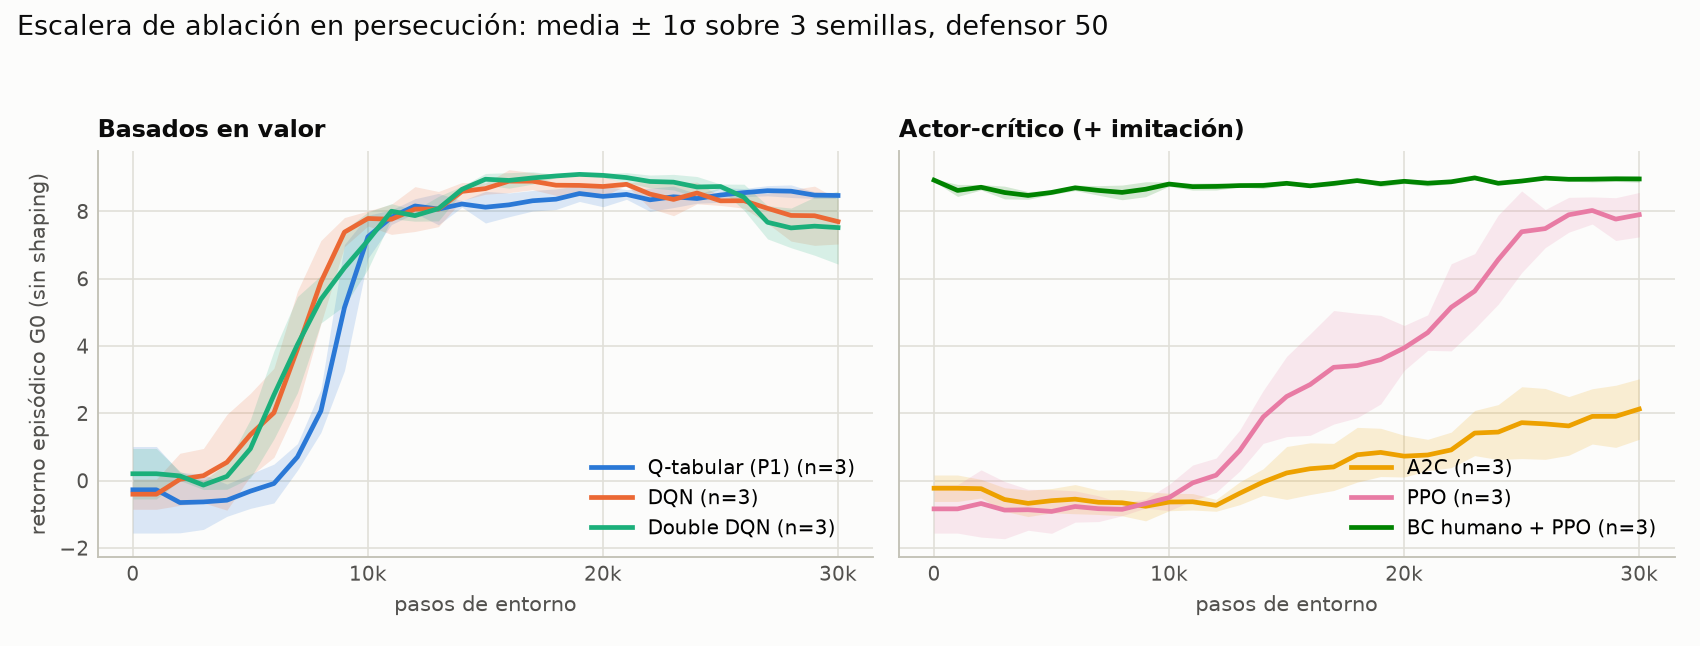
\includegraphics[width=0.92\textwidth]{pilar3_curvas.png}
\caption{Retorno episódico $\G$ (recompensa base, sin shaping) en persecución, media
$\pm1\sigma$ sobre 3 semillas. Todas las variantes usan PBRS durante el entrenamiento.}
\label{fig:curvas}
\end{figure*}

\begin{table}[t]
\centering
\caption{Escalera en persecución (3 semillas, 30k pasos, defensor 50). $\G$ asintótico =
media del último 20\,\% de episodios; $t_{80}$ = pasos hasta el 80\,\% del rango de $\G$;
prueba = 600 episodios (200 por semilla).}
\label{tab:escalera}
\setlength{\tabcolsep}{3.5pt}
\begin{tabular}{lcccc}
\toprule
Método & $\G$ asint. & $\sigma_{\text{semillas}}$ & $t_{80}$ & Éxito prueba\\
\midrule
Q tabular (P1) & 8,55 & 0,08 & 10,0k & ---\\
DQN & 8,14 & 0,34 & \textbf{9,0k} & \textbf{99,8\,\%}\\
Double DQN & 8,26 & 0,22 & 10,3k & 97,0\,\%\\
A2C & 2,25 & 0,80 & no llega & 72,0\,\%\\
PPO & 7,92 & 0,58 & 25,0k & 98,7\,\%\\
BC humano + PPO & \textbf{8,99} & \textbf{0,01} & \textbf{0} & \textbf{99,8\,\%}\\
\midrule
PPO sin shaping & 3,93 & 1,71 & no llega & 64,2\,\%\\
PPO shaping ingenuo & 2,47 & 1,20 & no llega & 40,5\,\%\\
\bottomrule
\end{tabular}
\end{table}

La Fig.~\ref{fig:curvas} y la Tabla~\ref{tab:escalera} muestran que, con el mismo presupuesto,
los métodos de valor fuera de política (DQN, DDQN) convergen en $\approx$10k pasos gracias
a que reutilizan la experiencia del \emph{replay}. PPO alcanza el mismo nivel, pero
necesita 2,5 veces más pasos. A2C, con una sola pasada por rollout y sin recorte, no
converge en 30k pasos y es el más inestable entre semillas ($\sigma=0{,}80$).
El Q tabular resuelve persecución porque la tarea es casi
de bajo dimensión (distancia y ángulo al balón). La escalera solo muestra ventaja de las
redes en las tareas con más jugadores (conducción y definición, $|s|=34$), que el tabular
no puede representar.
Arrancar desde BC humano elimina la fase de exploración ($t_{80}=0$) y reduce la varianza
entre semillas en dos órdenes de magnitud.

\begin{figure*}[t]
\centering
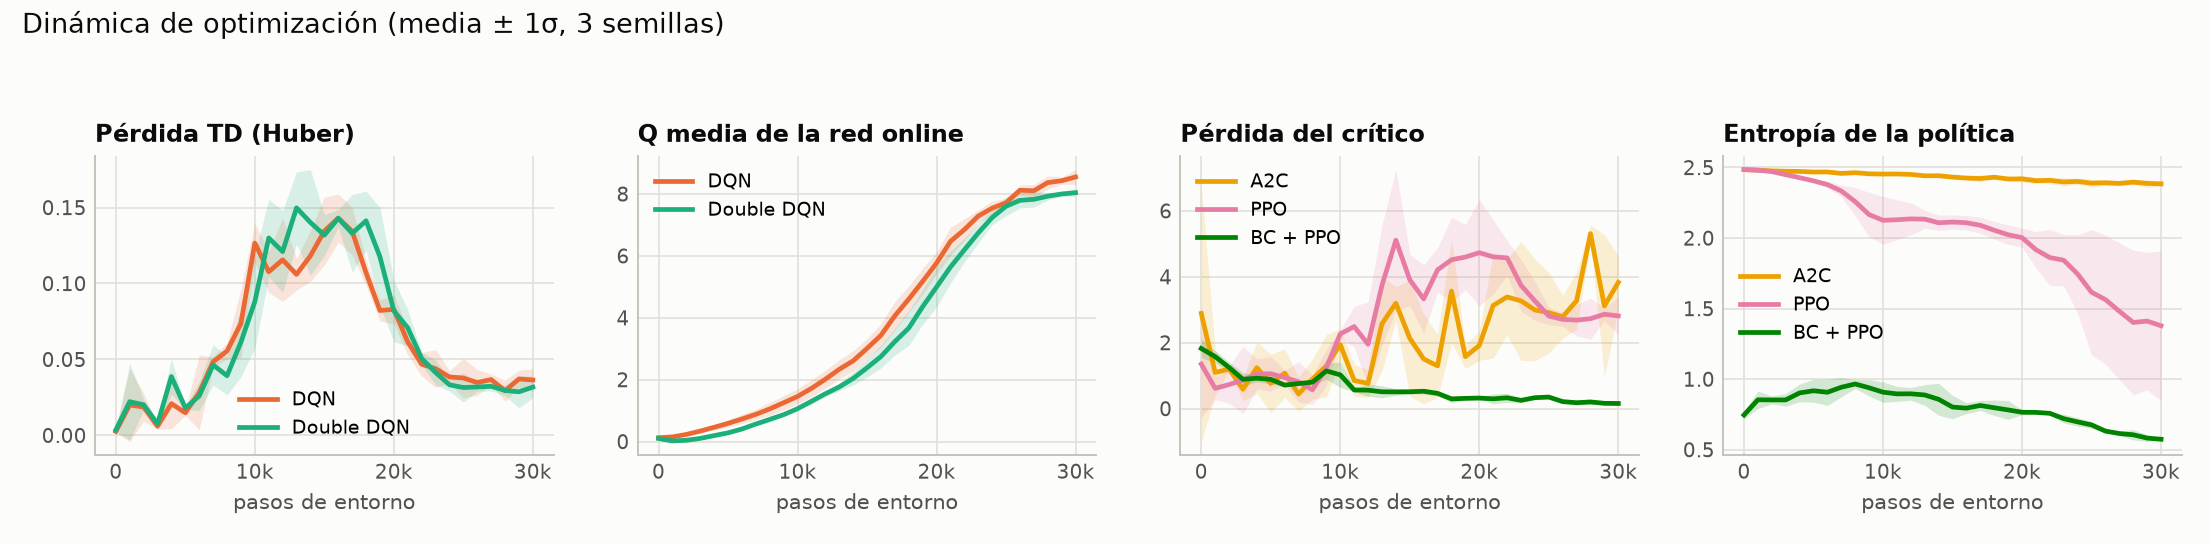
\includegraphics[width=0.97\textwidth]{pilar3_perdidas.png}
\caption{Dinámica de optimización (media $\pm1\sigma$, 3 semillas). La Q media de DQN
queda por encima de la de Double DQN, la firma de la sobreestimación por el $\max$.}
\label{fig:perdidas}
\end{figure*}

La Fig.~\ref{fig:perdidas} muestra la pérdida TD de DQN y DDQN, que crece mientras la
política mejora y aparecen recompensas $+10$, y luego cae. La Q media de DQN supera de
forma sostenida a la de DDQN, como predice \cite{vanhasselt2016}. Sin embargo, esa
corrección no se traduce en mejor éxito en esta tarea (97,0\,\% frente a 99,8\,\%). En PPO
la entropía decrece de forma monótona; en A2C apenas baja, lo que es coherente con su
lentitud.

\subsection{PBRS frente a shaping ingenuo (Pilar 2)}
\begin{figure*}[t]
\centering
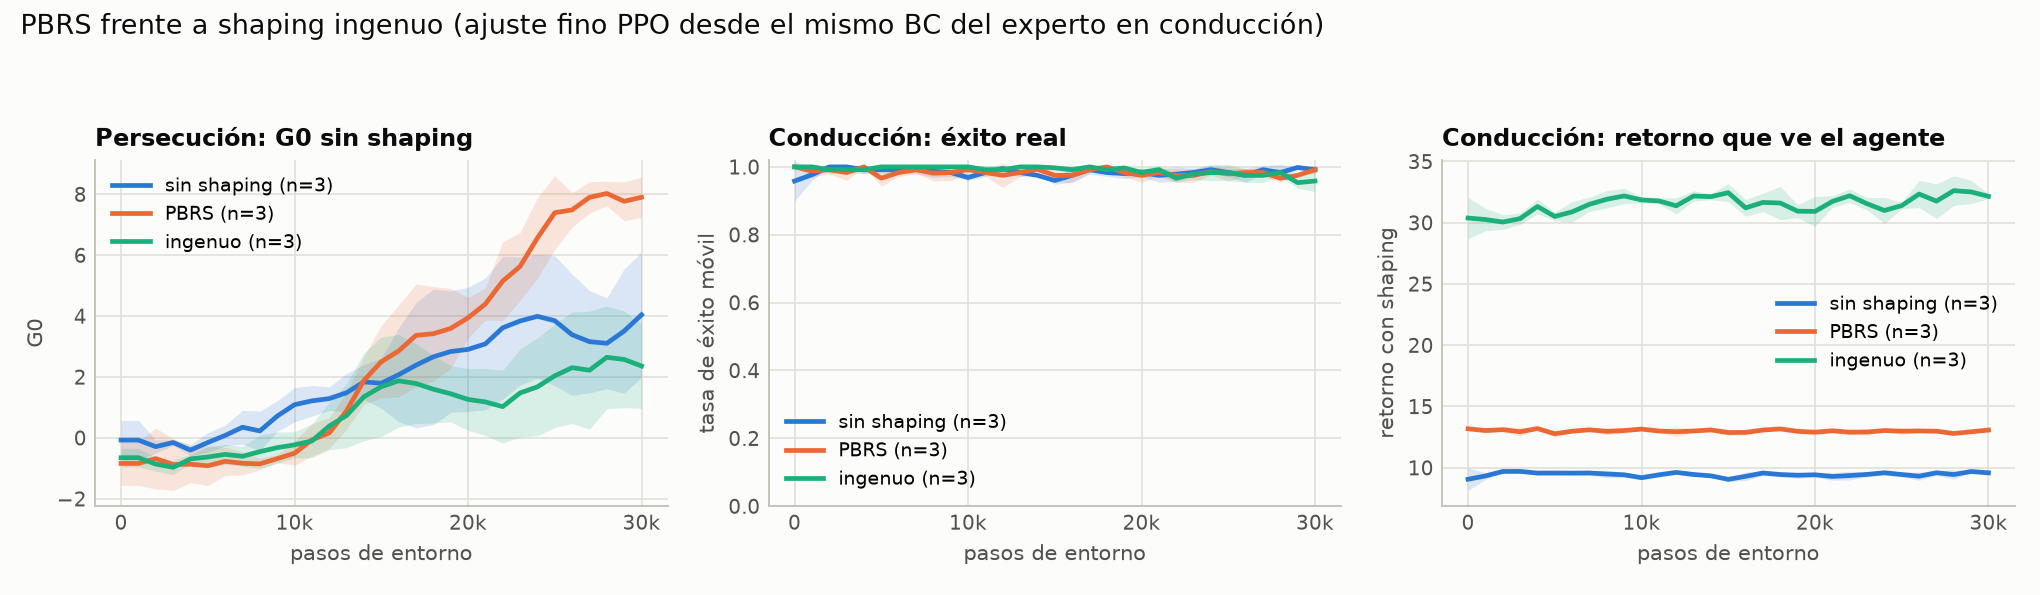
\includegraphics[width=0.97\textwidth]{pilar2_shaping.png}
\caption{Izq.: persecución desde cero. Centro y der.: ajuste fino PPO en conducción desde el
\emph{mismo} BC del experto. El shaping ingenuo infla el retorno que optimiza el agente
($\approx$32 frente a 13) mientras su éxito real baja: \emph{reward hacking}.}
\label{fig:shaping}
\end{figure*}

En persecución (Fig.~\ref{fig:shaping}, izq.), PBRS llega a 98,7\,\% de éxito en prueba,
frente a 64,2\,\% sin shaping y 40,5\,\% con el ingenuo (600 episodios por brazo; $z\geq15$, $p<10^{-6}$ en ambos casos).
El shaping ingenuo es peor que no usar shaping. En conducción, partiendo del mismo BC, el
shaping ingenuo hace que el agente vea un retorno 2,5 veces mayor, pero su éxito en prueba
cae de 99,2\,\% (PBRS) a 92,7\,\% (600 episodios por brazo, $z=5{,}7$, $p<10^{-7}$). Es
\emph{reward hacking}: se cobra por empujar el balón hacia delante aunque se pierda.
Con PBRS el retorno con shaping es solo un desplazamiento del base, por la Ec.~(1).

\subsection{Imitación y ajuste fino por habilidad}
\begin{table}[t]
\centering
\caption{Éxito por habilidad en prueba (200 episodios, defensor 50). Definición = gol.}
\label{tab:habilidades}
\setlength{\tabcolsep}{4pt}
\begin{tabular}{lccc}
\toprule
Variante & Persec. & Conducción & Definición\\
\midrule
BC humano & 100 & 13,0 & 57,5\\
DAgger humano & 100 & 53,5 & 58,0\\
BC experto programado & --- & 99,5 & ---\\
DAgger experto programado & --- & \textbf{100} & ---\\
Imitación + PPO & 100 & 98,0 & 63,5\\
Imitación + A2C & 100 & 100 & 52,0\\
Imitación + DQN (Double) & 100 & 70,5 & 83,0\\
DAgger + PPO (zona de tiro) & --- & --- & \textbf{86,0}\\
\bottomrule
\end{tabular}
\end{table}

La Tabla~\ref{tab:habilidades} resume la imitación. En conducción, la calidad del experto
domina: BC humano logra 13\,\%, porque el humano reacciona tarde al defensor y las
demostraciones son pocas e inconsistentes. DAgger humano corrige parte del
\emph{covariate shift} y sube a 53,5\,\% ($p<10^{-15}$). El experto programado, consistente
y etiquetando todos los estados, lleva BC y DAgger a $\geq$99,5\,\%. En definición, el ajuste
fino con RL aporta: la imitación queda en 58\,\% y el ajuste con Double DQN sube a 83\,\%, y PPO entrenado desde la distribución de
inicio que realmente ve en la jerarquía ($x\in[32,42]$, $y\in[-9,9]$, defensor cerca) llega a
86\,\%. El ajuste fino de DQN en conducción, en cambio, desestabiliza la política (70,5\,\%
frente a $\geq$98\,\% de PPO y A2C).

\subsection{Sistema jerárquico, Vía A}
\begin{figure}[t]
\centering
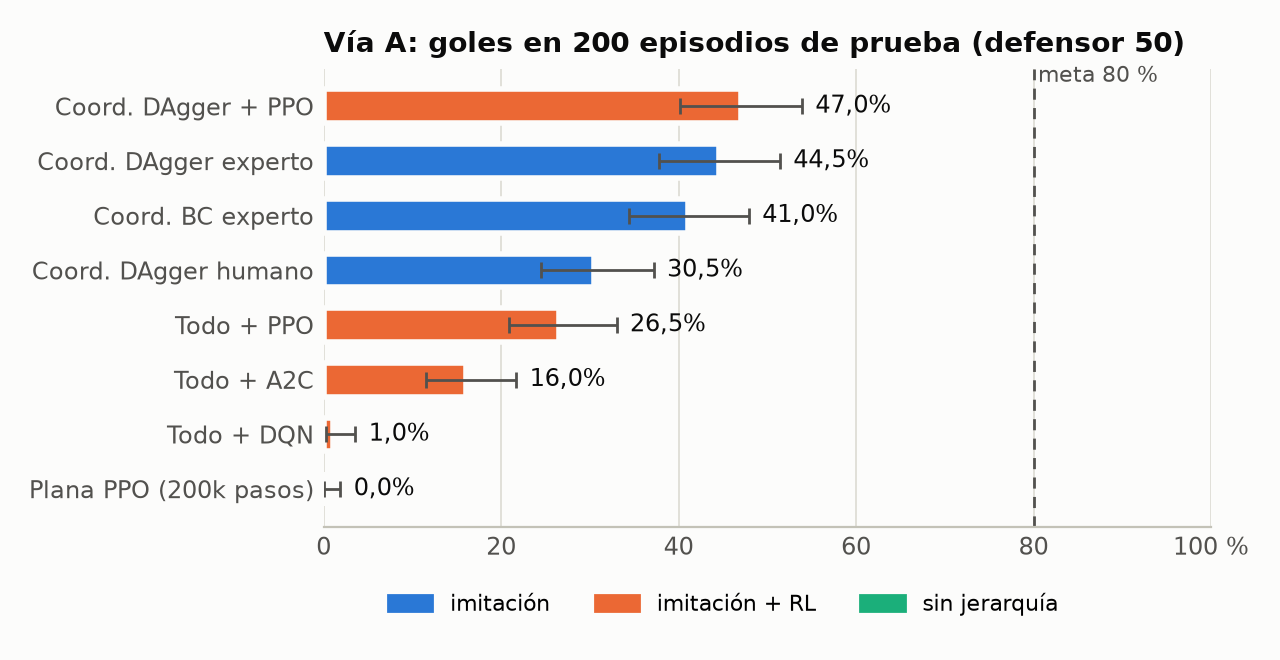
\includegraphics[width=\columnwidth]{jerarquia_final.png}
\caption{Goles del ataque completo 2v1 (200 episodios, IC Wilson 95\,\%).}
\label{fig:jerarquia}
\end{figure}

La Fig.~\ref{fig:jerarquia} compara coordinadores sobre habilidades congeladas. La primera
jerarquía (coordinador DAgger humano, opciones fijas de 8 ciclos) marca 30,5\,\%.
Ajustar con RL todo el sistema la empeora: 26,5\,\% con PPO, 16\,\% con A2C y 1\,\% con DQN.
El sistema final combina tres cambios: terminación $\beta(s)$ de opciones, definición
reentrenada en la zona de tiro y un coordinador aprendido por BC/DAgger del experto
programado más 15k decisiones de PPO. Marca \textbf{47,0\,\%} (IC 40,2--53,9\,\%), mejora
significativa sobre la primera jerarquía ($z=3{,}4$, $p<10^{-3}$). La política plana PPO,
entrenada desde cero 200k pasos en la misma condición, no marca ningún gol (0/200):
sin la descomposición, la recompensa de gol es demasiado escasa para descubrirla. Las etapas BC (41,0\,\%) $\to$ DAgger (44,5\,\%) $\to$ +PPO (47,0\,\%) mejoran
de forma monótona, pero cada paso por separado no es significativo con $n=200$
($p>0{,}4$). \textbf{La meta del 80\,\% no se alcanza.}

\section{Discusión crítica}
\textbf{¿Por qué no llega al 80\,\%?} Se registró la causa de fin de 200 episodios del
coordinador DAgger en el script de diagnóstico. El 44\,\% de los episodios termina con el
rival en posesión, casi siempre el arquero tras atajar o despejar el tiro (última opción
activa: persecución tras disparar). El 21,5\,\% se agota el tiempo con conducción activa y
el balón detenido cerca de $x\approx38$. En el 34\,\% restante hubo gol. El cuello de
botella no es el coordinador: el experto de reglas que imita obtiene el mismo nivel
(42,5\,\% en el diagnóstico). El problema es la \emph{composición} de las habilidades.
Definición convierte el 86\,\% cuando se inicia desde su distribución de entrenamiento, pero
dentro de la jerarquía recibe el balón en estados peores: en movimiento, mal orientado y con
el defensor encima. Es un \emph{distribution shift} entre habilidades que ninguna habilidad
congelada ve durante su entrenamiento.

\textbf{Por qué falló el ajuste fino global.} Ajustar con RL las habilidades y el coordinador
a la vez vuelve no estacionario el problema del coordinador, y el crédito de un gol se reparte
entre pocas decisiones de alto nivel (10--15 por episodio). DQN, además, sobreajusta al
\emph{replay} reciente en tareas de recompensa escasa. Esto reproduce la conocida
fragilidad de ajustar con RL una política iniciada por imitación sin regularización hacia la
política de referencia (KL o \emph{behavior cloning} auxiliar).

\textbf{Vías de mejora.} (i)~Entrenar definición con estados iniciales tomados de los
traspasos reales de la jerarquía (o \emph{curriculum}); (ii)~ajustar conducción para
entregar el balón quieto y orientado (una recompensa terminal de ``buen pase a
definición''); (iii)~entrenar de extremo a extremo con opciones aprendidas (option-critic)
o RL del coordinador con regularización KL hacia DAgger; (iv)~aumentar $n$ para separar
diferencias de 3--5 puntos.

\textbf{Limitaciones.} Estado privilegiado (no percepción parcial), acciones discretas
sobre física continua, compañero y rivales heurísticos, una sola condición de prueba
(defensor 50) y RNG físico no fijable. El tabular solo se compara en persecución.

\section{Conclusiones}
Con implementaciones propias en PyTorch, la escalera muestra que DQN/DDQN son los más
eficientes en muestras en esta tarea, PPO es estable pero lento y A2C es el más frágil.
PBRS acelera el aprendizaje y es seguro, mientras que el shaping ingenuo es peor que no usar
shaping y provoca \emph{reward hacking} medible. La imitación de un experto consistente con
DAgger es la palanca más fuerte: conducción pasa de 13\,\% a 100\,\%. La jerarquía Vía~A
mejora de 30,5\,\% a 47,0\,\% de goles, pero queda lejos del 80\,\%. El límite está en el
traspaso entre habilidades, no en el coordinador ni en las habilidades aisladas.

\bibliographystyle{IEEEtran}
\begin{thebibliography}{10}
\bibitem{sutton1999options} R.~S. Sutton, D.~Precup y S.~Singh, ``Between MDPs and semi-MDPs: A framework for temporal abstraction in reinforcement learning,'' \emph{Artif. Intell.}, vol.~112, pp.~181--211, 1999.
\bibitem{mnih2015} V.~Mnih \emph{et~al.}, ``Human-level control through deep reinforcement learning,'' \emph{Nature}, vol.~518, pp.~529--533, 2015.
\bibitem{vanhasselt2016} H.~van Hasselt, A.~Guez y D.~Silver, ``Deep reinforcement learning with double Q-learning,'' en \emph{AAAI}, 2016.
\bibitem{mnih2016} V.~Mnih \emph{et~al.}, ``Asynchronous methods for deep reinforcement learning,'' en \emph{ICML}, 2016.
\bibitem{schulman2016gae} J.~Schulman, P.~Moritz, S.~Levine, M.~Jordan y P.~Abbeel, ``High-dimensional continuous control using generalized advantage estimation,'' en \emph{ICLR}, 2016.
\bibitem{schulman2017} J.~Schulman, F.~Wolski, P.~Dhariwal, A.~Radford y O.~Klimov, ``Proximal policy optimization algorithms,'' arXiv:1707.06347, 2017.
\bibitem{ng1999} A.~Y. Ng, D.~Harada y S.~Russell, ``Policy invariance under reward transformations: Theory and application to reward shaping,'' en \emph{ICML}, 1999.
\bibitem{ross2011} S.~Ross, G.~Gordon y D.~Bagnell, ``A reduction of imitation learning and structured prediction to no-regret online learning,'' en \emph{AISTATS}, 2011.
\bibitem{kelly2019} M.~Kelly, C.~Sidrane, K.~Driggs-Campbell y M.~J. Kochenderfer, ``HG-DAgger: Interactive imitation learning with human experts,'' en \emph{ICRA}, 2019.
\bibitem{hester2018} T.~Hester \emph{et~al.}, ``Deep Q-learning from demonstrations,'' en \emph{AAAI}, 2018.
\bibitem{noda1998} I.~Noda, H.~Matsubara, K.~Hiraki e I.~Frank, ``Soccer server: A tool for research on multiagent systems,'' \emph{Appl. Artif. Intell.}, vol.~12, pp.~233--250, 1998.
\end{thebibliography}

\end{document}
